\problem{Lunacy}

\begin{wrapfigure}{r}{0.25\linewidth}
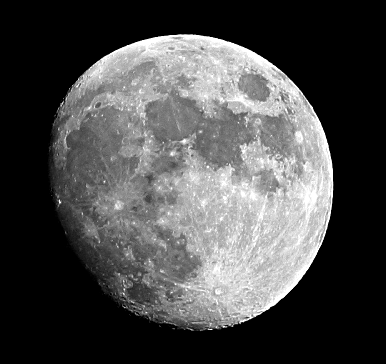
\includegraphics[width=\linewidth]{moon/moon_2.png}
\end{wrapfigure}
After several months struggling with a diet, Jack has become obsessed
with the idea of weighing less. In an odd way, he finds it very
comforting to think that, if he had simply had the luck to be born on
a different planet, his weight could be considerably less.

Of course, the planets are far out of reach, but even the Earth's moon
would yield a dramatic weight loss. Objects on the moon weight only
0.167 of their weight on Earth.

\subsection*{Input}

Input consists of one or more lines, each containing a single floating
point number denoting a weight (in pounds) on the Earth. The end of
input is denoted by a negative floating point number.


\subsection*{Output}

For each line of input data, your program should print a single line
of the form
\begin{alltt}
X Y
\end{alltt}
where \texttt{X} is the weight from the input and \texttt{Y} is the
corresponding weight on the moon. Both output numbers should be
printed to a precision of 2 digits after the decimal point. The
numbers should be separated on the line by a single blank.

\subsection*{Example}
\subsubsection*{Input:}
\verbfile{moon/test0.in}
\subsubsection*{Output:}
\verbfile{moon/test0.expected}



